\documentclass[tikz,border=8pt]{standalone}
\usepackage[utf8]{inputenc}
\usepackage[T1]{fontenc}
\usepackage{amsmath}
\usetikzlibrary{arrows.meta,positioning,fit,backgrounds,calc}

\tikzset{
  >=Latex,
  fixed/.style={draw, rounded corners, fill=blue!8, align=center,
    minimum height=8mm, text width=37mm, font=\scriptsize},
  hyper/.style={draw, rounded corners, fill=violet!10, align=center,
    minimum height=9mm, text width=42mm, font=\scriptsize},
  latent/.style={draw, circle, fill=white, align=center,
    minimum size=13mm, font=\scriptsize},
  observed/.style={draw, rounded corners, fill=black!12, align=center,
    minimum height=9mm, text width=34mm, font=\scriptsize},
  det/.style={draw, rounded corners, fill=yellow!16, align=center,
    minimum height=9mm, text width=35mm, font=\scriptsize},
  dateplate/.style={draw, rounded corners, dashed, inner sep=3.5mm},
  arr/.style={-{Latex[length=2mm]}, line width=.55pt},
  weakarr/.style={-{Latex[length=2mm]}, line width=.45pt, dashed}
}

\begin{document}
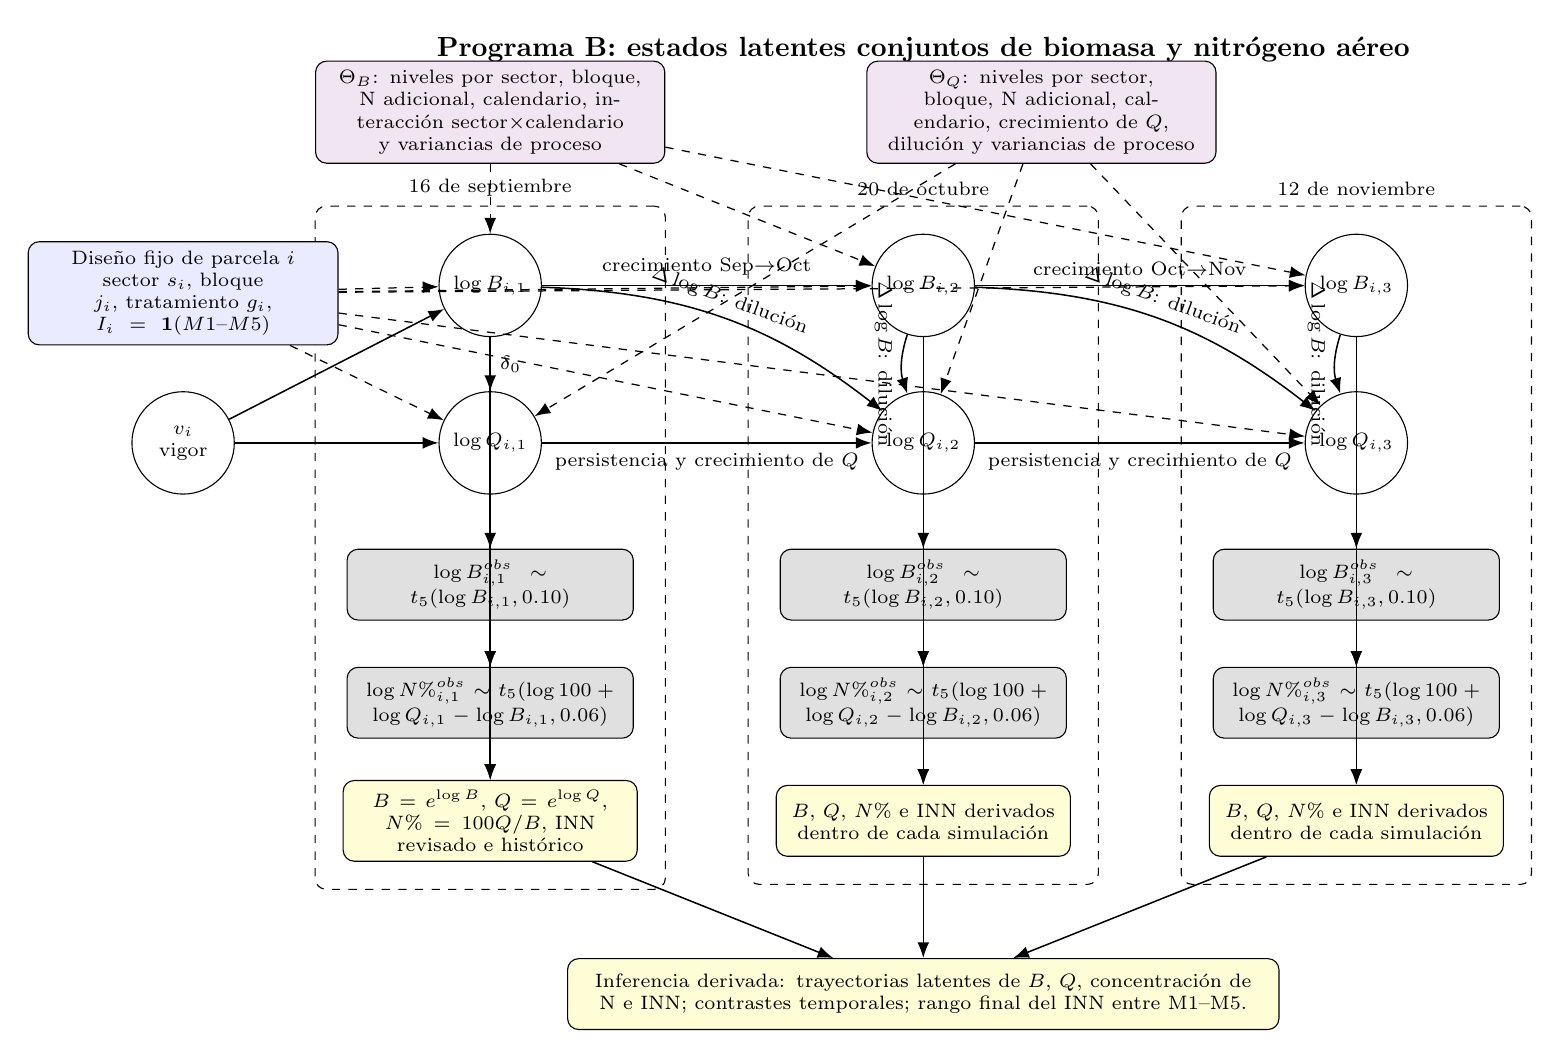
\begin{tikzpicture}[x=1cm,y=1cm]
\node[font=\bfseries] at (6.7,6.8)
  {Programa B: estados latentes conjuntos de biomasa y nitrógeno aéreo};

\node[fixed] (design) at (-2.7,3.7)
  {Diseño fijo de parcela $i$\\sector $s_i$, bloque $j_i$, tratamiento $g_i$, $I_i=\mathbf 1(M1\text{--}M5)$};
\node[latent] (vigor) at (-2.7,1.8) {$v_i$\\vigor};
\node[hyper] (thetaB) at (1.2,6.0)
  {$\Theta_B$: niveles por sector, bloque, N adicional, calendario, interacción sector$\times$calendario y variancias de proceso};
\node[hyper] (thetaQ) at (8.2,6.0)
  {$\Theta_Q$: niveles por sector, bloque, N adicional, calendario, crecimiento de $Q$, dilución y variancias de proceso};

% September
\node[latent] (B1) at (1.2,3.8) {$\log B_{i,1}$};
\node[latent] (Q1) at (1.2,1.8) {$\log Q_{i,1}$};
\node[observed] (Bobs1) at (1.2,0.0)
  {$\log B^{obs}_{i,1}\sim t_5(\log B_{i,1},0.10)$};
\node[observed] (Nobs1) at (1.2,-1.5)
  {$\log N\%^{obs}_{i,1}\sim t_5(\log100+\log Q_{i,1}-\log B_{i,1},0.06)$};
\node[det] (D1) at (1.2,-3.0)
  {$B=e^{\log B}$, $Q=e^{\log Q}$, $N\%=100Q/B$, INN revisado e histórico};

% October
\node[latent] (B2) at (6.7,3.8) {$\log B_{i,2}$};
\node[latent] (Q2) at (6.7,1.8) {$\log Q_{i,2}$};
\node[observed] (Bobs2) at (6.7,0.0)
  {$\log B^{obs}_{i,2}\sim t_5(\log B_{i,2},0.10)$};
\node[observed] (Nobs2) at (6.7,-1.5)
  {$\log N\%^{obs}_{i,2}\sim t_5(\log100+\log Q_{i,2}-\log B_{i,2},0.06)$};
\node[det] (D2) at (6.7,-3.0)
  {$B$, $Q$, $N\%$ e INN derivados dentro de cada simulación};

% November
\node[latent] (B3) at (12.2,3.8) {$\log B_{i,3}$};
\node[latent] (Q3) at (12.2,1.8) {$\log Q_{i,3}$};
\node[observed] (Bobs3) at (12.2,0.0)
  {$\log B^{obs}_{i,3}\sim t_5(\log B_{i,3},0.10)$};
\node[observed] (Nobs3) at (12.2,-1.5)
  {$\log N\%^{obs}_{i,3}\sim t_5(\log100+\log Q_{i,3}-\log B_{i,3},0.06)$};
\node[det] (D3) at (12.2,-3.0)
  {$B$, $Q$, $N\%$ e INN derivados dentro de cada simulación};

% Fixed design and hyperparameters
\foreach \n in {B1,Q1,B2,Q2,B3,Q3}{\draw[weakarr] (design) -- (\n);}
\draw[arr] (vigor) -- (B1);
\draw[arr] (vigor) -- (Q1);
\foreach \n in {B1,B2,B3}{\draw[weakarr] (thetaB) -- (\n);}
\foreach \n in {Q1,Q2,Q3}{\draw[weakarr] (thetaQ) -- (\n);}

% State transitions
\draw[arr] (B1) -- node[above, font=\scriptsize]{crecimiento Sep$\to$Oct} (B2);
\draw[arr] (B2) -- node[above, font=\scriptsize]{crecimiento Oct$\to$Nov} (B3);
\draw[arr] (Q1) -- node[below, font=\scriptsize]{persistencia y crecimiento de $Q$} (Q2);
\draw[arr] (Q2) -- node[below, font=\scriptsize]{persistencia y crecimiento de $Q$} (Q3);
\draw[arr, bend left=18] (B1) to node[above, sloped, font=\scriptsize]{$\Delta\log B$: dilución} (Q2);
\draw[arr, bend right=18] (B2) to node[below, sloped, font=\scriptsize]{$\Delta\log B$: dilución} (Q2);
\draw[arr, bend left=18] (B2) to node[above, sloped, font=\scriptsize]{$\Delta\log B$: dilución} (Q3);
\draw[arr, bend right=18] (B3) to node[below, sloped, font=\scriptsize]{$\Delta\log B$: dilución} (Q3);
\draw[arr] (B1) -- node[right, font=\scriptsize]{$\delta_0$} (Q1);

% Observation and deterministic nodes
\foreach \b/\bo in {B1/Bobs1,B2/Bobs2,B3/Bobs3}{\draw[arr] (\b) -- (\bo);}
\draw[arr] (B1) -- (Nobs1); \draw[arr] (Q1) -- (Nobs1);
\draw[arr] (B2) -- (Nobs2); \draw[arr] (Q2) -- (Nobs2);
\draw[arr] (B3) -- (Nobs3); \draw[arr] (Q3) -- (Nobs3);
\draw[arr] (B1) -- (D1); \draw[arr] (Q1) -- (D1);
\draw[arr] (B2) -- (D2); \draw[arr] (Q2) -- (D2);
\draw[arr] (B3) -- (D3); \draw[arr] (Q3) -- (D3);

% Date plates
\begin{scope}[on background layer]
  \node[dateplate, fit=(B1)(Q1)(Bobs1)(Nobs1)(D1),
    label={[font=\scriptsize]above:16 de septiembre}] {};
  \node[dateplate, fit=(B2)(Q2)(Bobs2)(Nobs2)(D2),
    label={[font=\scriptsize]above:20 de octubre}] {};
  \node[dateplate, fit=(B3)(Q3)(Bobs3)(Nobs3)(D3),
    label={[font=\scriptsize]above:12 de noviembre}] {};
\end{scope}

\node[det, text width=88mm] (out) at (6.7,-5.2)
  {Inferencia derivada: trayectorias latentes de $B$, $Q$, concentración de N e INN; contrastes temporales; rango final del INN entre M1--M5.};
\draw[arr] (D1) -- (out);
\draw[arr] (D2) -- (out);
\draw[arr] (D3) -- (out);

\end{tikzpicture}
\end{document}
